\begin{figure}[H]
    \centering
    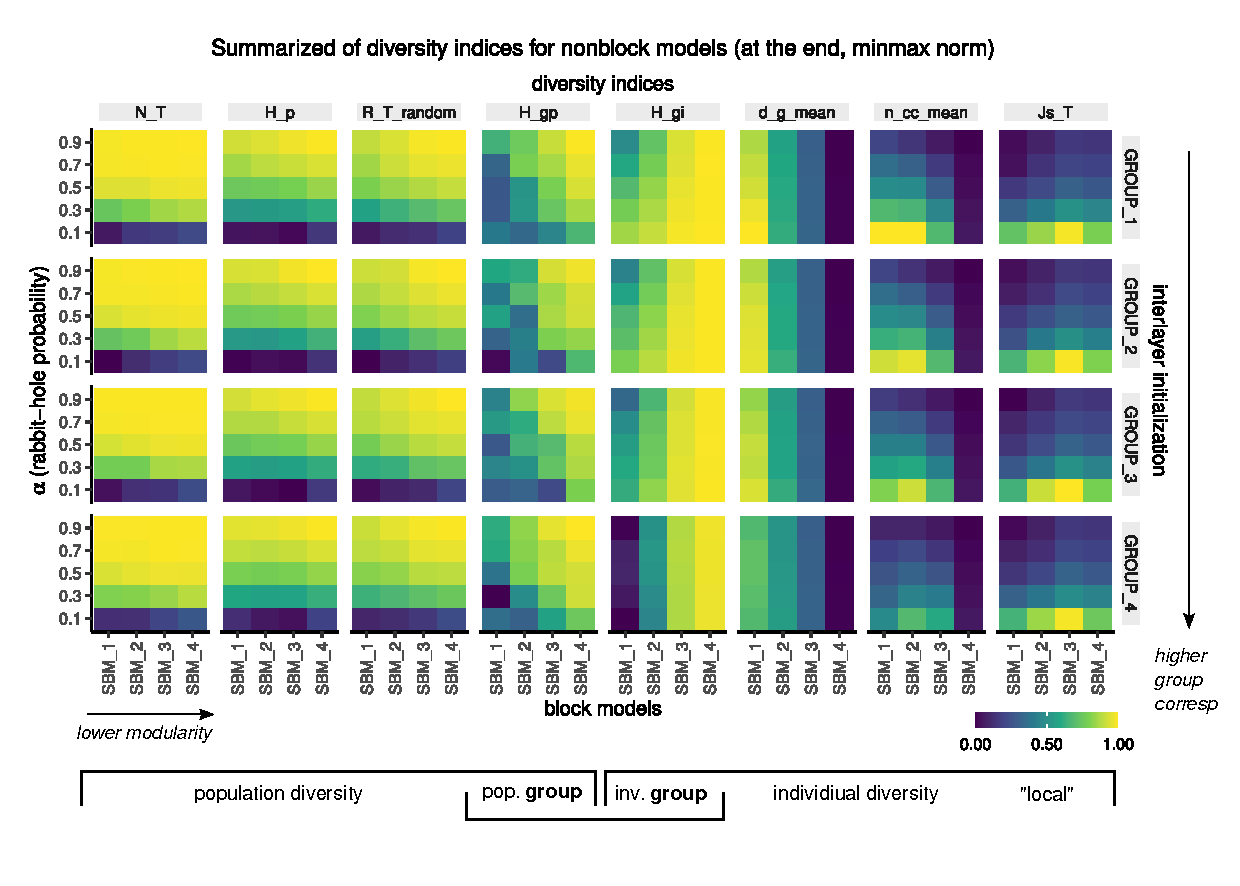
\includegraphics[width=0.95\textwidth,center]{../figures/report/Fig6.pdf}
    \caption{\label{fig:6}
    \textit{Summary  of  population  and  individual  diversity  indices  due  to $\alpha$,  across  different  block  models}. Within each panel, x-axis shows decreasing modularity of intralayer model, y-axis is $\alpha$ while the color represents values here at the end of the simulation, and min-max normalized within each metric. From left to right are different diversity metrics (see text for more information). From top to bottom are different group correspondence initialization strategies (top is equivalent to a random initialization; see \autoref{supp:2} for example)
    }
\end{figure}